\documentclass[notes,10pt, aspectratio=169]{beamer}

\usepackage{pgfpages}
% These slides also contain speaker notes. You can print just the slides,
% just the notes, or both, depending on the setting below. Comment out the want
% you want.
\setbeameroption{hide notes} % Only slide
%\setbeameroption{show only notes} % Only notes
%\setbeameroption{show notes on second screen=right} % Both
\usepackage{wrapfig}

\usepackage{helvet}
\usepackage[default]{lato}
\usepackage{array}
\usepackage{eurosym}
\usepackage{setspace}
\usepackage{animate}
\usepackage{multicol}
\usepackage{breqn}
\usepackage{subcaption}
\usepackage{caption}
\captionsetup{font=scriptsize, justification=raggedright,singlelinecheck=false}
\usepackage[export]{adjustbox}
\usepackage[scale=2]{ccicons}
\usepackage{tikz}
\newenvironment{wideitemize}{\itemize\addtolength{\itemsep}{10pt}}{\enditemize}
\usepackage{natbib}

\usepackage{tikz}
\usepackage{verbatim}
\setbeamertemplate{note page}{\pagecolor{yellow!5}\insertnote}
\usepackage{amsmath}
%\usepackage{mathpazo}
\usepackage{hyperref}
\usepackage{lipsum}
\usepackage{multimedia}
\usepackage{multirow}
\usepackage{graphicx}
\usepackage{dcolumn}
\usepackage{bbm}
\newcolumntype{d}[0]{D{.}{.}{5}}

\usepackage{changepage}
\usepackage{appendixnumberbeamer}
% \newcommand{\beginbackup}{
%   \newcounter{framenumbervorappendix}
%   \setcounter{framenumbervorappendix}{\value{framenumber}}
%   \setbeamertemplate{footline}
%   {
%      \leavevmode%
%      \hline
%      box{%
%       \begin{beamercolorbox}[wd=\paperwidth,ht=2.25ex,dp=1ex,right]{footlinecolor}%
% %         \insertframenumber  \hspace*{2ex} 
%       \end{beamercolorbox}}%
%      \vskip0pt%
%   }
%  }
\useinnertheme[shadow]{rounded}
\setbeamercolor{block title example}{fg=black,bg=orange!50!white}
\setbeamercolor{block body example}{fg=black, bg=orange!30!white}
\setbeamercolor{block title}{use=structure,fg=structure.fg,bg=structure.fg!20!bg}
\setbeamercolor{block body}{parent=normal text,use=block title,bg=block title.bg!50!bg}

 \setbeamertemplate{footline}{
    \hbox{%
    \begin{beamercolorbox}[wd=\paperwidth,ht=3ex,dp=1.5ex,leftskip=2ex,rightskip=2ex]{page footer}%
        %\usebeamerfont{title in head/foot}%
        %\insertshorttitle \hfill
        %\insertsection \hfill
        %\tableofcontents[currentsection] \hfill
        \insertsectionnavigationhorizontal{0.7\paperwidth}{}{} \hfill 
        \insertframenumber{} / \inserttotalframenumber
    \end{beamercolorbox}}%
}
\newcommand{\backupend}{
   \addtocounter{framenumbervorappendix}{-\value{framenumber}}
   \addtocounter{framenumber}{\value{framenumbervorappendix}} 
}


\usepackage{graphicx}
\usepackage[space]{grffile}
\usepackage{booktabs}

% These are my colors -- there are many like them, but these ones are mine.
\definecolor{blue}{RGB}{0,114,178}
\definecolor{red}{RGB}{213,94,0}
\definecolor{yellow}{RGB}{240,228,66}
\definecolor{green}{RGB}{0,158,115}

\setbeamercolor{section in head/foot}{fg=blue}


\hypersetup{
  colorlinks=false,
  linkbordercolor = {white},
  linkcolor = {blue}
}


%% I use a beige off white for my background
\definecolor{MyBackground}{RGB}{255,253,218}

%% Uncomment this if you want to change the background color to something else
%\setbeamercolor{background canvas}{bg=MyBackground}

%% Change the bg color to adjust your transition slide background color!
\newenvironment{transitionframe}{
  \setbeamercolor{background canvas}{bg=yellow}
  \begin{frame}}{
    \end{frame}
}

\setbeamercolor{frametitle}{fg=blue}
\setbeamercolor{title}{fg=black}
%\setbeamertemplate{footline}[frame number]
\setbeamertemplate{navigation symbols}{} 
\setbeamertemplate{itemize items}{-}
\setbeamercolor{itemize item}{fg=blue}
\setbeamercolor{itemize subitem}{fg=blue}
\setbeamercolor{enumerate item}{fg=blue}
\setbeamercolor{enumerate subitem}{fg=blue}
\setbeamercolor{button}{bg=white,fg=blue,}



% If you like road maps, rather than having clutter at the top, have a roadmap show up at the end of each section 
% (and after your introduction)
% Uncomment this is if you want the roadmap!
% \AtBeginSection[]
% {
%    \begin{frame}
%        \frametitle{Roadmap of Talk}
%        \tableofcontents[currentsection]
%    \end{frame}
% }

\useinnertheme[shadow]{rounded}
\setbeamercolor{block title example}{fg=black,bg=orange!50!white}
\setbeamercolor{block body example}{fg=black, bg=orange!30!white}
\setbeamercolor{block title}{use=structure,fg=structure.fg,bg=structure.fg!20!bg}
\setbeamercolor{block body}{parent=normal text,use=block title,bg=block title.bg!50!bg}


\setbeamercolor{section in toc}{fg=blue}
\setbeamercolor{subsection in toc}{fg=red}
%\setbeamersize{text margin left=1em,text margin right=1em} 
\setbeamersize{text margin left=0.7cm,text margin right=0.7cm} 


\title[]{\textcolor{blue}{Lecture 4 v2:\\OLS Implementation}}
\author{25117 - Econometrics}
\institute[shortinst]{Universitat Pompeu Fabra}

\date{October 9th, 2024}

\begin{document}



% Title Slide

\begin{frame}[plain]
\maketitle
\end{frame}

\section{Introduction}

\begin{frame}{What we learned in the last lesson}
\begin{itemize}
    \item The population regression line, $\beta_0 + \beta_1 X$, is the mean of $Y$ as a function of the value of $X$.
    \begin{itemize}
        \item The slope, $\beta_1$, is the expected difference in $Y$ between two observations with $X$ values that differ by one unit.
        \item The intercept, $\beta_0$, determines the level (or height) of the regression line.
    \end{itemize}\vspace{1em}
    \item The population regression line can be estimated using sample observations $(Y_i, X_i)$ with $i = 1, \dots, n$ by ordinary least squares (OLS).
    \begin{itemize}
        \item The OLS estimators of the regression intercept and slope are denoted $\hat{\beta}_0$ and $\hat{\beta}_1$.
        \item The predicted value of Y given X is $\hat{Y}=\hat{\beta}_0 + \hat{\beta}_1 X$.
    \end{itemize}\vspace{1em}
\end{itemize}
\end{frame}

\begin{frame}{What we learned in the last lesson}
\begin{itemize}
    \item The $R^2$ and standard error of the regression (SER) are measures of how close the values of $Y_i$ are to the estimated regression line.\\
    \begin{itemize}
        \item The $R^2$ is between 0 and 1, indicating how much variance in our outcome is explained by the variance of our regressors.
        \item The standard error of the regression estimates the standard deviation of the regression error.
    \end{itemize}
    \vspace{1em}
    \item There are three key assumptions for estimating causal effects using the linear regression model:
    \begin{enumerate}
        \item The regression errors, $u_i$, have a mean of 0, conditional on the regressors $X_i$;
        \item the sample observations are i.i.d. random draws from the population; and 
        \item large outliers are unlikely
    \end{enumerate}
    \vspace{1em}
   \item If these assumptions hold, the OLS estimator $\hat{\beta}_1$ is 
    \begin{enumerate}
        \item  an unbiased estimator of the causal effect ${\beta}_1$
        \item consistent
        \item normally distributed when the sample is large.
    \end{enumerate}
\end{itemize}
\end{frame}



\begin{frame}{Estimation of the regression line}
We want to learn about the slope of the population regression line. We have data from a sample, so there is sampling uncertainty. There are five steps toward this goal:
    \begin{enumerate}
        \item State the population of interest 
        \item Provide an estimator of this population object
        \item Derive the sampling distribution of the estimator (this requires certain assumptions). In large samples, this sampling distribution will be normal by the CLT.
        \item The square root of the estimated variance of the sampling distribution is the standard error (SE) of the estimator
        \item Use the SE to construct t-statistics (for hypothesis tests) and confidence intervals.
    \end{enumerate}
\end{frame}


\begin{frame}{Estimation of the regression line}
 \begin{columns}
\begin{column}{0.35\textwidth}
$Y_i = \beta_0 + \beta_1 X_i + u_i$\\\vspace{.5cm}
    \begin{itemize}
        \item $\beta_1$ is the slope of the population regression line
        \item $\hat{\beta}_1$ is the OLS estimator of $\beta_1$
         \item Under homoskedasticity and the usual regularity conditions, the large-sample distribution conditional on $X$ is approximately $\mathcal{N}(\beta_1; \sigma_u^2/TSS_X)$.
    \end{itemize}
\end{column}
\begin{column}{0.62\textwidth}
\begin{figure}
  \centering
         \vspace{-5mm}
        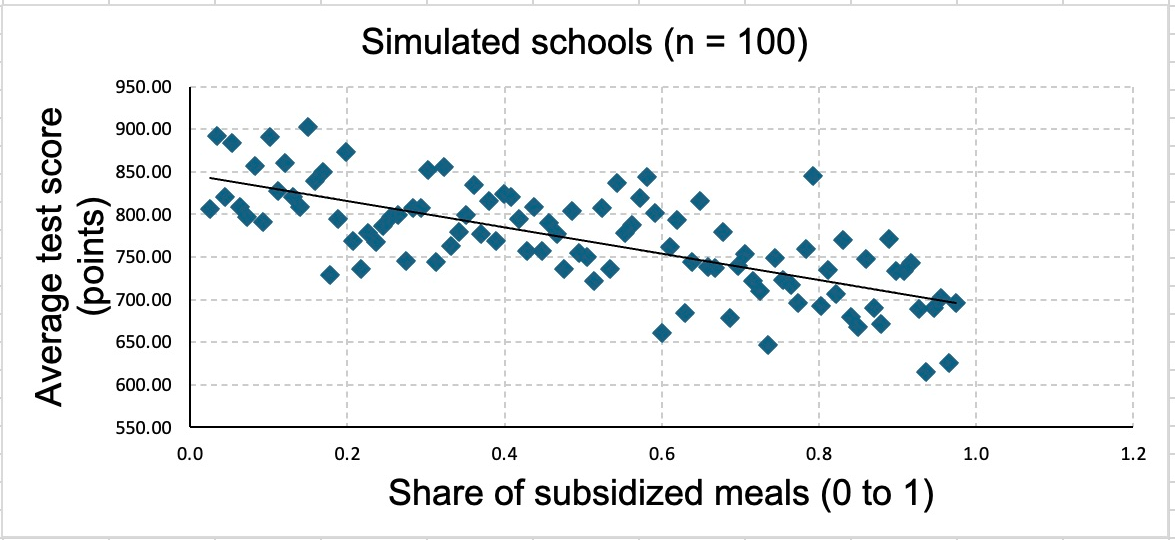
\includegraphics[width=\linewidth]{images/lecture4_excel_scatter.png}
\end{figure}
\end{column}
\end{columns}
\end{frame}


\begin{frame}{Hypothesis Testing}
 \begin{columns}
\begin{column}{0.35\textwidth}
    \begin{itemize}
        \item Most of the time, we test for $H_0: \beta_1=0$
        \item Null hypothesis and two-sided alternative:
        \begin{itemize}
            \item $H_0: \beta_1=\beta_{1,0} \text{~~~~vs.~~~~} H_1: \beta_1\neq\beta_{1,0}$ 
        \end{itemize}
        \item Null hypothesis and one-sided alternative:
        \begin{itemize}
            \item $H_0: \beta_1=\beta_{1,0} \text{~~~~vs.~~~~} H_1: \beta_1 < (or >)\beta_{1,0}$ 
        \end{itemize}
    \end{itemize}
\end{column}
\begin{column}{0.62\textwidth}
\begin{figure}
  \centering
         \vspace{-5mm}
        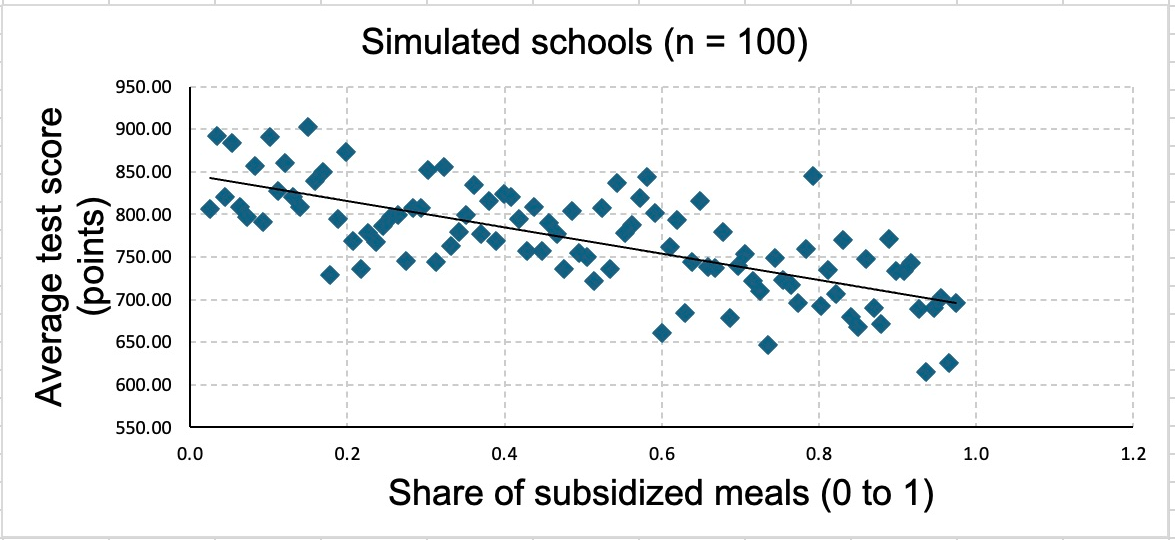
\includegraphics[width=\linewidth]{images/lecture4_excel_scatter.png}
\end{figure}
\end{column}
\end{columns}
\end{frame}

\begin{frame}{Hypothesis Testing}
    \begin{itemize}
        \item In general, the t-statistic is given by
        \begin{equation*}
            t=\frac{\text{estimator}-\text{hypothetised value}}{\text{standard error of the estimator}}
        \end{equation*}
        \item For $\mu_{Y}$, the t-statistic is given by
        \begin{equation*}
            t=\frac{\overline{Y}-\mu_{Y,0}}{s_Y/\sqrt{n}}
        \end{equation*}
        \item For $\beta_1$, the t-statistic is given by
        \begin{equation*}
            t=\frac{\hat{\beta}_1-\beta_{1,0}}{SE(\hat{\beta}_1)}
        \end{equation*}
        where $SE(\hat{\beta}_1)=\sqrt{\frac{SSR}{(n-2) TSS_X}}=\sqrt{\frac{\sum_{i=1}^n \hat{u}_i^2}{(n-2)\sum_{i=1}^n (X_i-\overline{X})^2}}$ when errors are homoskedastic (i.e., $var(u_i\mid X)=\sigma^2_u$~~~$\forall i=1,\dots, n$)
        \item Using the large-sample normal approximation, reject $H_0: \beta_1=\beta_{1,0}$ at 5\% if $|t|>1.96$, or if the two-sided $p$-value is below $0.05$. Excel's finite-sample test uses a $t_{n-2}$ critical value instead.

    \end{itemize}
\end{frame}

\begin{frame}{Excel: A Dataset of 100 Simulated Schools}
\small
Open \texttt{Lecture4\_Excel\_100schools.xlsx}, sheet \textbf{Data}.
\begin{columns}[T]
\begin{column}{.27\textwidth}
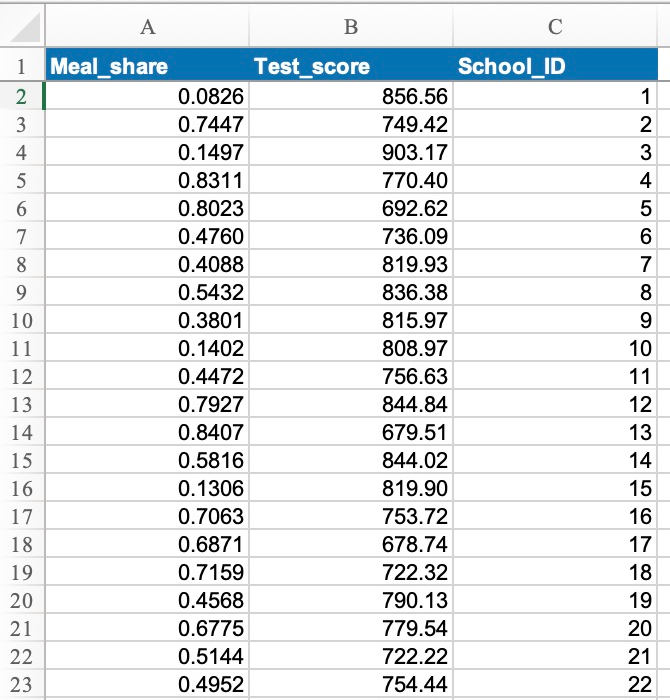
\includegraphics[width=\linewidth,height=4.1cm,keepaspectratio]{images/lecture4_excel_data_table.png}
\end{column}
\begin{column}{.69\textwidth}
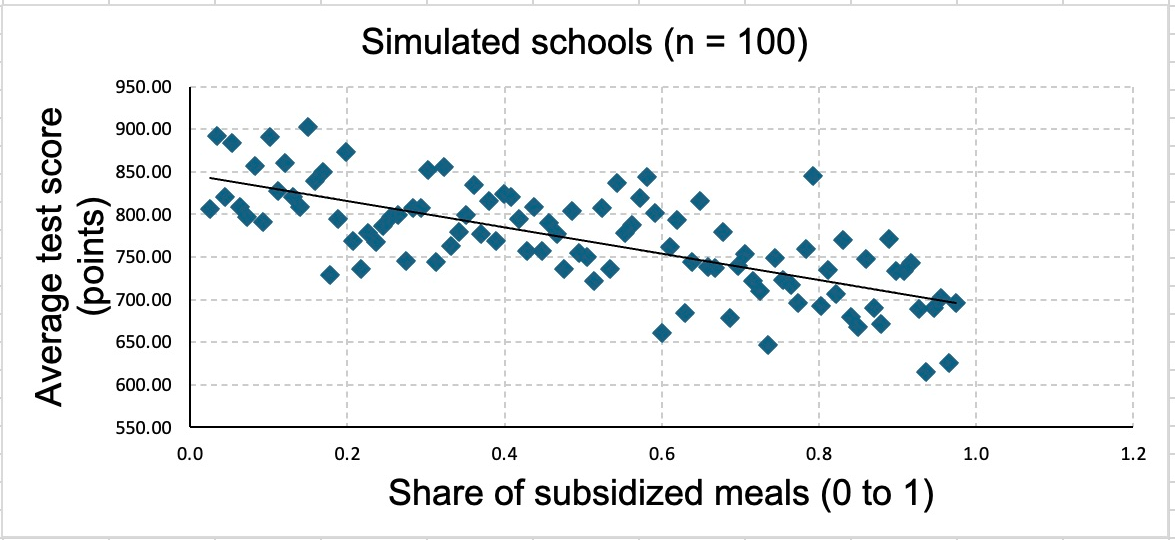
\includegraphics[width=\linewidth]{images/lecture4_excel_scatter.png}
\end{column}
\end{columns}
\begin{itemize}
\item $X_i$: share of subsidized meals (0--1). $Y_i$: average test score, in points.
\item These are \textbf{simulated teaching data}, with a negative association similar to the earlier example. They are not the original school records.
\end{itemize}
\end{frame}

\begin{frame}{Excel Step 1: Enable the Analysis ToolPak}
\small
\begin{enumerate}
\item In desktop Excel, enable \textbf{Analysis ToolPak} if \textbf{Data Analysis} is missing:
\begin{itemize}
\item \textbf{Mac:} Tools $\rightarrow$ Excel Add-ins $\rightarrow$ Analysis ToolPak $\rightarrow$ OK.
\item \textbf{Windows:} File $\rightarrow$ Options $\rightarrow$ Add-ins; Manage: Excel Add-ins $\rightarrow$ Go. Check Analysis ToolPak and click OK.
\end{itemize}
\item Open the \textbf{Data} tab and click \textbf{Data Analysis}.
\end{enumerate}
\begin{center}
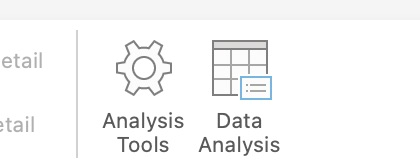
\includegraphics[width=5.8cm]{images/lecture4_excel_data_button.png}
\end{center}
The screenshots show Excel for Mac. The regression input ranges and calculations are the same on Windows.
\par\medskip
{\scriptsize Setup reference: \href{https://support.microsoft.com/en-us/excel/load-the-analysis-toolpak-in-excel}{Microsoft: Load the Analysis ToolPak in Excel}.}
\end{frame}

\begin{frame}{Excel Step 2: Choose Regression}
\begin{columns}[c]
\begin{column}{.44\textwidth}
\begin{enumerate}
\item In the list of analysis tools, select \textbf{Regression}.
\item Click \textbf{OK}.
\end{enumerate}
\medskip
We want Excel to estimate
\[
Y_i=\beta_0+\beta_1X_i+u_i
\]
by minimizing the sum of squared residuals.
\end{column}
\begin{column}{.52\textwidth}
\centering
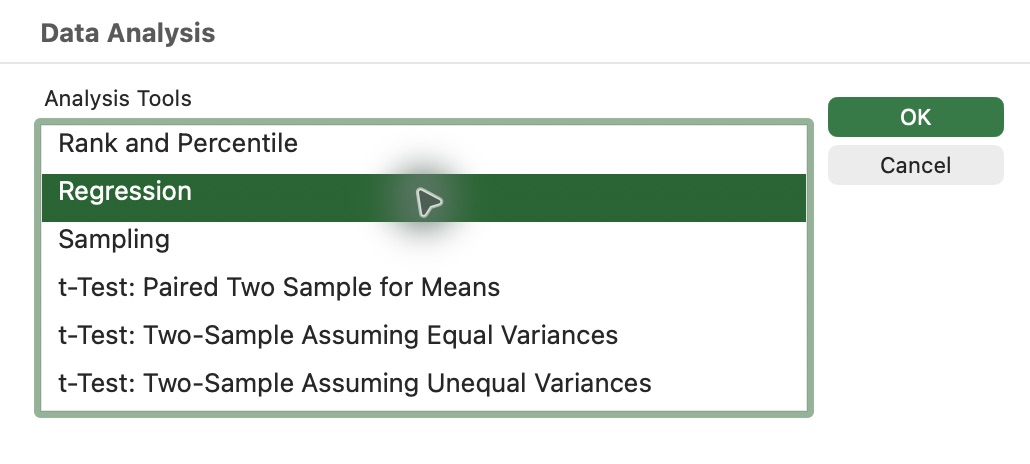
\includegraphics[width=\linewidth,height=5.4cm,keepaspectratio]{images/lecture4_excel_choose_regression.png}
\end{column}
\end{columns}
\end{frame}

\begin{frame}{Excel Step 3: Set the Input Ranges}
\begin{columns}[c]
\begin{column}{.47\textwidth}
\small
\begin{enumerate}
\item \textbf{Input Y Range:}\\
\texttt{Data!\$B\$1:\$B\$101}\\
The outcome is \textbf{Test\_score}.
\item \textbf{Input X Range:}\\
\texttt{Data!\$A\$1:\$A\$101}\\
The explanatory variable is \textbf{Meal\_share}.
\item Check \textbf{Labels}: row 1 contains names, so there are 100 observations.
\item Leave \textbf{Constant is Zero} unchecked: estimate an intercept.
\end{enumerate}
\end{column}
\begin{column}{.49\textwidth}
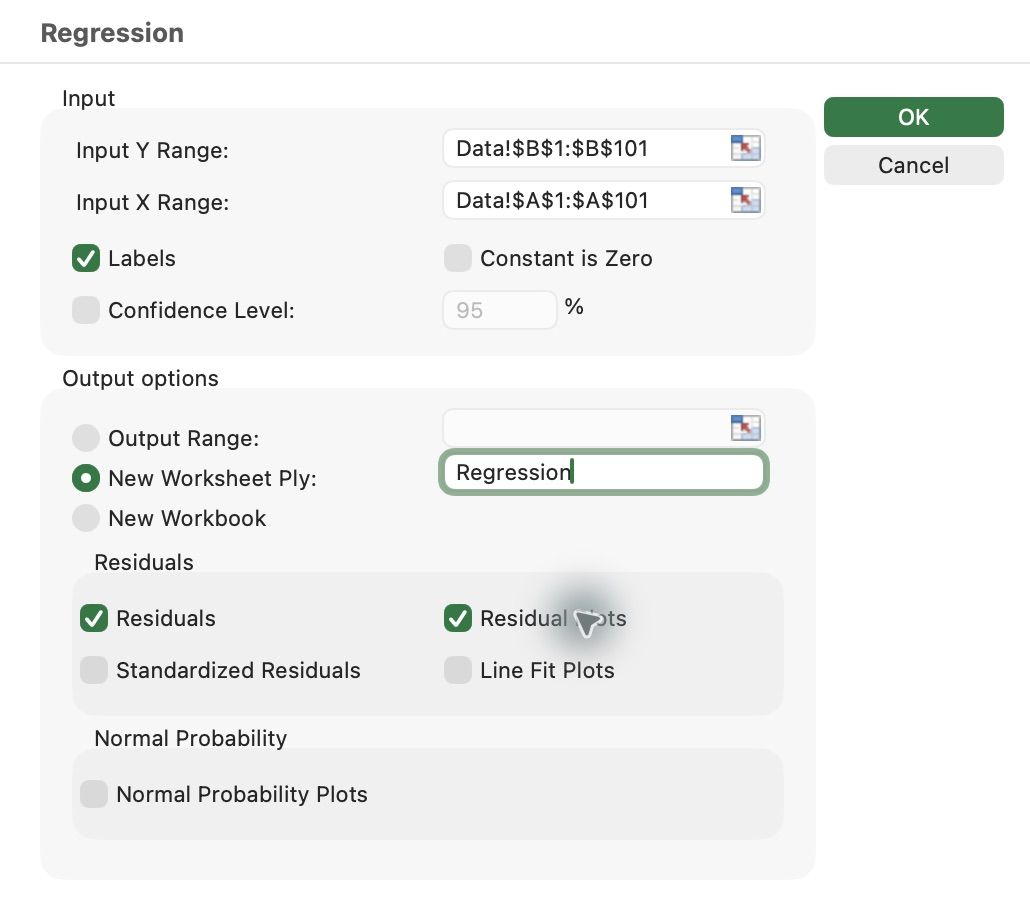
\includegraphics[width=\linewidth,height=5.7cm,keepaspectratio]{images/lecture4_excel_settings.png}
\end{column}
\end{columns}
\end{frame}

\begin{frame}{Excel Step 4: Choose the Output}
\begin{columns}[c]
\begin{column}{.47\textwidth}
\small
\begin{enumerate}
\item Choose \textbf{New Worksheet Ply} and name it \textbf{Regression}. If that sheet already exists, use a new name, such as \textbf{Regression2}.
\item Check \textbf{Residuals} and \textbf{Residual Plots}.
\item The output includes \textbf{95\% confidence intervals} by default.
\item Click \textbf{OK}. Widen the output columns if numbers are cut off.
\end{enumerate}
\medskip
ToolPak output is a \textbf{snapshot}: rerun the regression after changing the data.
\end{column}
\begin{column}{.49\textwidth}
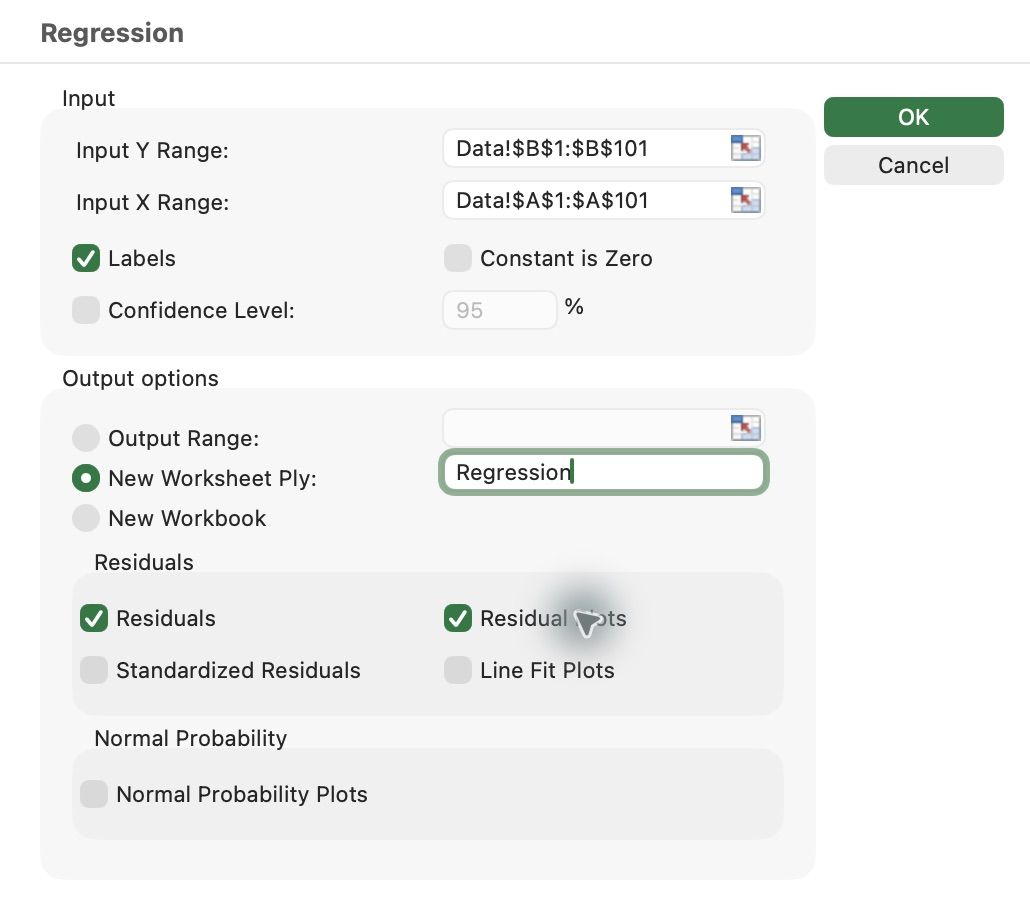
\includegraphics[width=\linewidth,height=5.7cm,keepaspectratio]{images/lecture4_excel_settings.png}
\end{column}
\end{columns}
\end{frame}

\begin{frame}{Excel Step 5: Read the Summary Output}
\centering
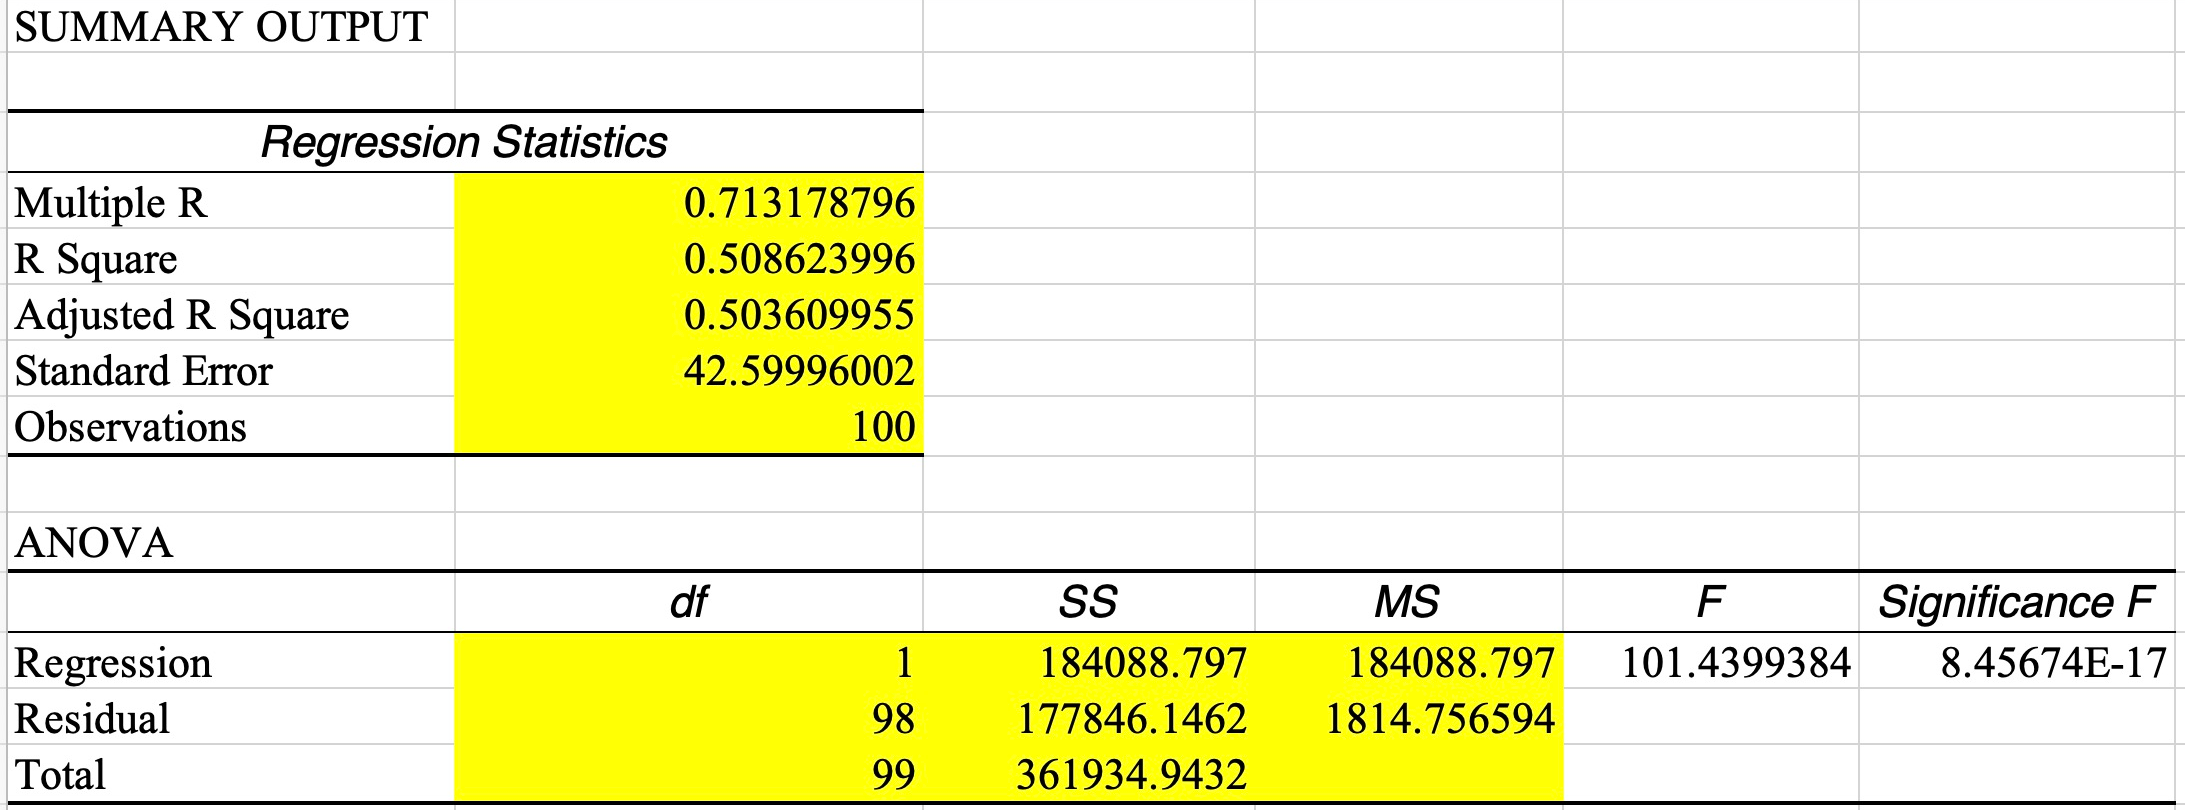
\includegraphics[width=.94\textwidth,height=4.1cm,keepaspectratio]{images/lecture4_excel_summary.png}
\par\medskip
\raggedright\small
\begin{itemize}
\item \textbf{Observations:} $n=100$. Two coefficients are estimated, so residual degrees of freedom are $100-2=98$.
\item \textbf{R Square:} $0.5086$. \textbf{Standard Error:} $42.60$, the SER.
\item Under ANOVA, \textbf{Residual SS} is our $SSR$; \textbf{Total SS} is $TSS_Y$.
\end{itemize}
Yellow cells identify the results discussed in these slides.
\end{frame}

\begin{frame}{Excel: Interpret the Estimated Coefficients}
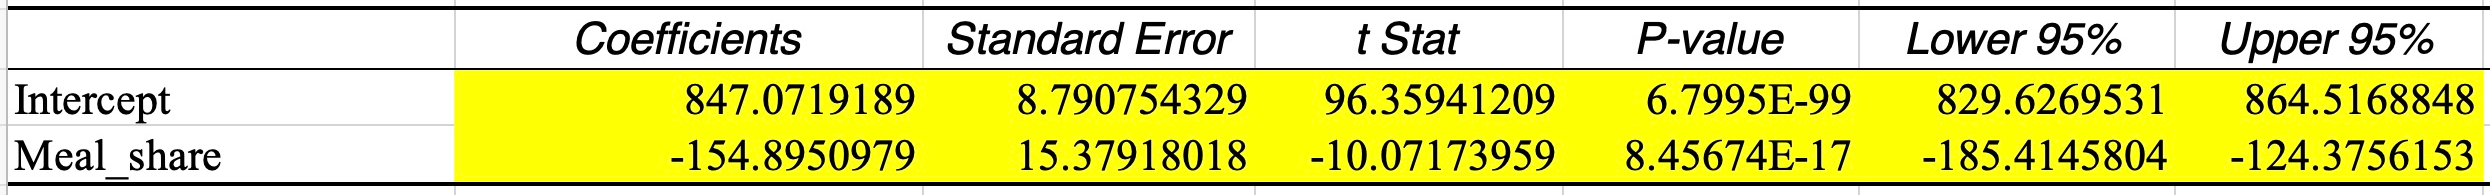
\includegraphics[width=\textwidth]{images/lecture4_excel_coefficients.png}
\[
\widehat Y_i=847.0719-154.8951X_i.
\]
\begin{itemize}
\item \textbf{Intercept:} the fitted score at $X=0$ is $847.07$. Since the simulated sample has $X>0$, this is an extrapolation.
\item \textbf{Slope:} increasing $X$ by $0.10$ (10 percentage points) is associated with a change of
\[
-154.8951\times0.10=-15.49\text{ test-score points}.
\]
\item An association alone does not establish a causal effect of subsidized meals.
\end{itemize}
\end{frame}

\begin{frame}{Excel: Test Whether Each Coefficient Is Zero}
\small
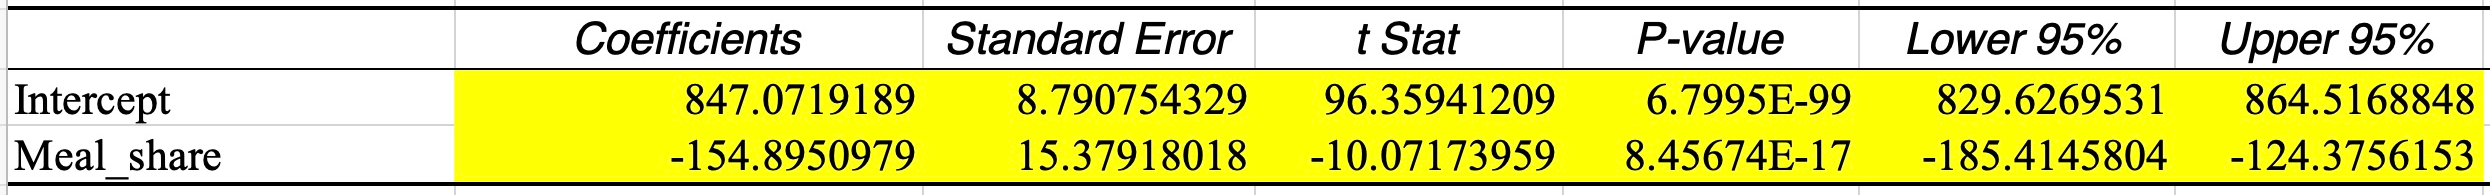
\includegraphics[width=\textwidth]{images/lecture4_excel_coefficients.png}
\[
H_0:\beta_j=0,\qquad
t_j=\frac{\widehat\beta_j-0}{SE(\widehat\beta_j)},\qquad
p_j=P\!\left(|T_{98}|\geq |t_j|\right).
\]
\begin{center}
\begin{tabular}{lrrr}
\toprule
Coefficient & Standard error & $t$ statistic & Two-sided $p$-value\\
\midrule
Intercept & 8.7908 & 96.3594 & $6.80\times10^{-99}$\\
Meal\_share & 15.3792 & $-10.0717$ & $8.46\times10^{-17}$\\
\bottomrule
\end{tabular}
\end{center}
Both $p$-values are below $0.05$: reject both zero-coefficient null hypotheses at 5\%.
These are very small probabilities, \textbf{not zero}.
\par\medskip
{\footnotesize ToolPak uses homoskedastic standard errors. Exact finite-sample $t_{98}$ inference also assumes conditionally normal errors, with independent observations and conditional mean zero.}
\end{frame}

\begin{frame}{Excel: Construct 95\% Confidence Intervals}
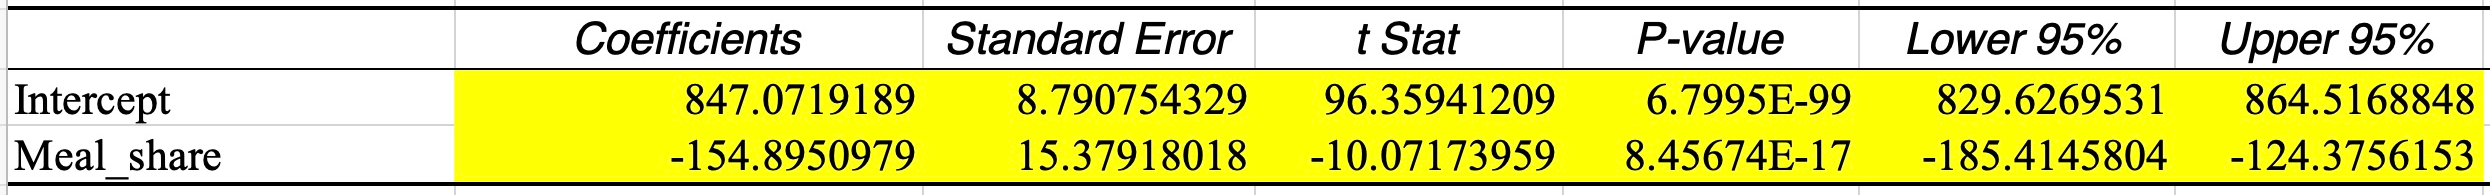
\includegraphics[width=\textwidth]{images/lecture4_excel_coefficients.png}
\[
\widehat\beta_j\ \pm\ t_{0.975,98}\,SE(\widehat\beta_j),
\qquad t_{0.975,98}=1.9845.
\]
\begin{align*}
CI_{\beta_0}&=847.0719\pm1.9845(8.7908)
             =[829.6270,\ 864.5169],\\
CI_{\beta_1}&=-154.8951\pm1.9845(15.3792)
             =[-185.4146,\ -124.3756].
\end{align*}
\small
\begin{itemize}
\item These are Excel's \textbf{Lower 95\%} and \textbf{Upper 95\%} columns (using unrounded values).
\item Neither interval contains zero, consistent with the two-sided tests.
\item In repeated sampling, 95\% of intervals constructed this way cover the true coefficient, under the stated assumptions.
\end{itemize}
\end{frame}

\begin{frame}{Excel: Standard Error, SER, and RMSE}
\small
First compute the fitted value and the residual:
\[
\widehat Y_i=\widehat\beta_0+\widehat\beta_1X_i,\qquad
\widehat u_i=Y_i-\widehat Y_i,\qquad
SSR=\sum_{i=1}^{100}\widehat u_i^2=177{,}846.1462.
\]
\begin{columns}[T]
\begin{column}{.48\textwidth}
\begin{block}{Excel's Standard Error = SER}
\[
SER=\sqrt{\frac{SSR}{n-2}}
=\sqrt{\frac{177{,}846.1462}{98}}
=42.6000.
\]
The denominator adjusts for estimating two coefficients. This estimates the error standard deviation.
\end{block}
\end{column}
\begin{column}{.48\textwidth}
\begin{block}{RMSE with denominator $n$}
\[
RMSE=\sqrt{\frac{SSR}{n}}
=\sqrt{\frac{177{,}846.1462}{100}}
=42.1718.
\]
This is the square root of the average squared prediction error within the sample.
\end{block}
\end{column}
\end{columns}
\medskip
Both are measured in \textbf{test-score points}. In this course, distinguish the denominators; the earlier Stata Root MSE label corresponds to the SER.
\end{frame}

\begin{frame}{Excel: Compute and Interpret $R^2$}
\small
\begin{align*}
TSS_Y&=\sum_i(Y_i-\overline Y)^2=361{,}934.9432,\\
SSR&=\sum_i(Y_i-\widehat Y_i)^2=177{,}846.1462,\\
ESS&=\sum_i(\widehat Y_i-\overline Y)^2=184{,}088.7970.
\end{align*}
With an intercept, $TSS_Y=ESS+SSR$. Therefore,
\[
R^2=1-\frac{SSR}{TSS_Y}
=1-\frac{177{,}846.1462}{361{,}934.9432}
=0.5086.
\]
\begin{itemize}
\item The fitted line explains \textbf{50.86\% of the sample variation} in test scores around their mean.
\item This measures in-sample fit, not the proportion of scores caused by meals.
\item Adjusted $R^2=1-(1-R^2)\frac{n-1}{n-2}=0.5036$ penalizes the use of a regressor.
\end{itemize}
\end{frame}

\begin{frame}{Excel: Inspect Predicted Values and Residuals}
\begin{columns}[T]
\begin{column}{.40\textwidth}
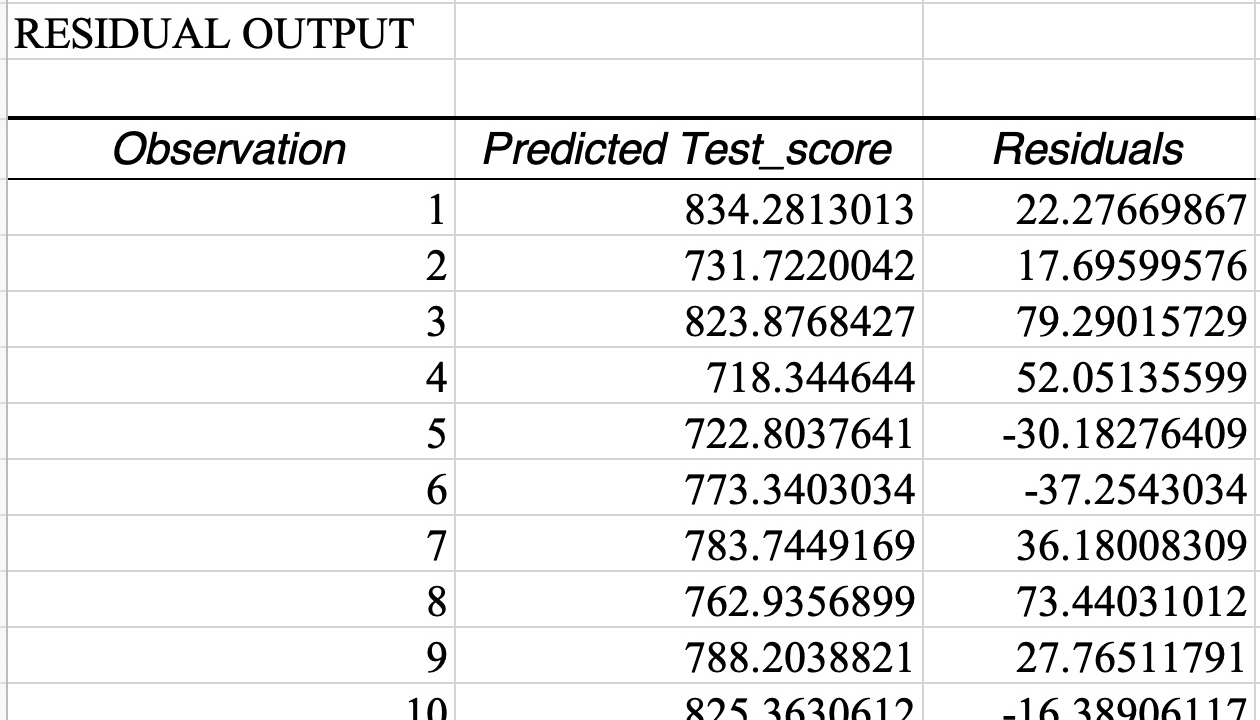
\includegraphics[width=\linewidth,height=3.6cm,keepaspectratio]{images/lecture4_excel_residuals.png}
\end{column}
\begin{column}{.56\textwidth}
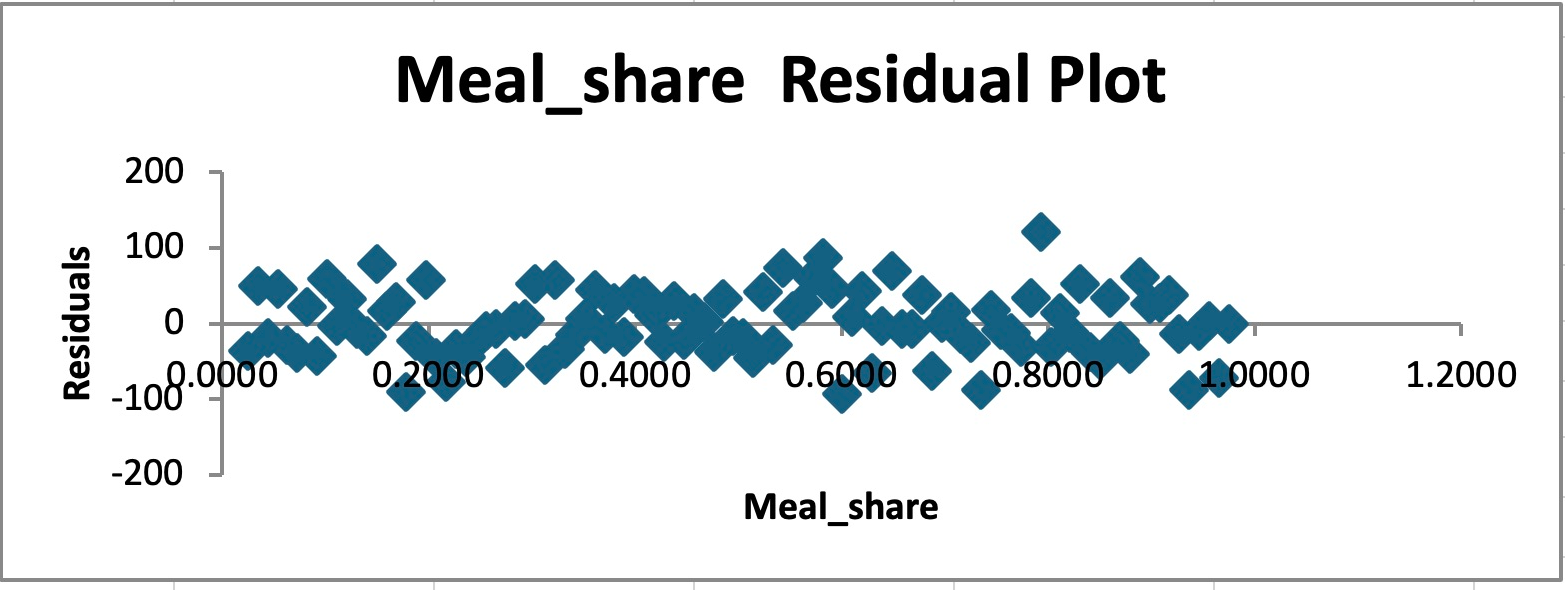
\includegraphics[width=\linewidth]{images/lecture4_excel_residual_plot.png}
\end{column}
\end{columns}
\small
For observation 1, $Y_1=856.5580$ and $\widehat Y_1=834.2813$, so
\[
\widehat u_1=Y_1-\widehat Y_1=22.2767.
\]
The model underpredicts this school's score by 22.28 points.
Look for patterns or changes in residual spread; a plot alone cannot prove homoskedasticity.
\end{frame}

\begin{frame}{By Hand, Step 1: Means and Deviations}
\small
Open \textbf{Paso\_a\_paso}. Each of the 100 observations has its own row (43--142).
\[
\overline X=\frac{\sum_iX_i}{100}=0.5000,\qquad
\overline Y=\frac{\sum_iY_i}{100}=769.6244.
\]
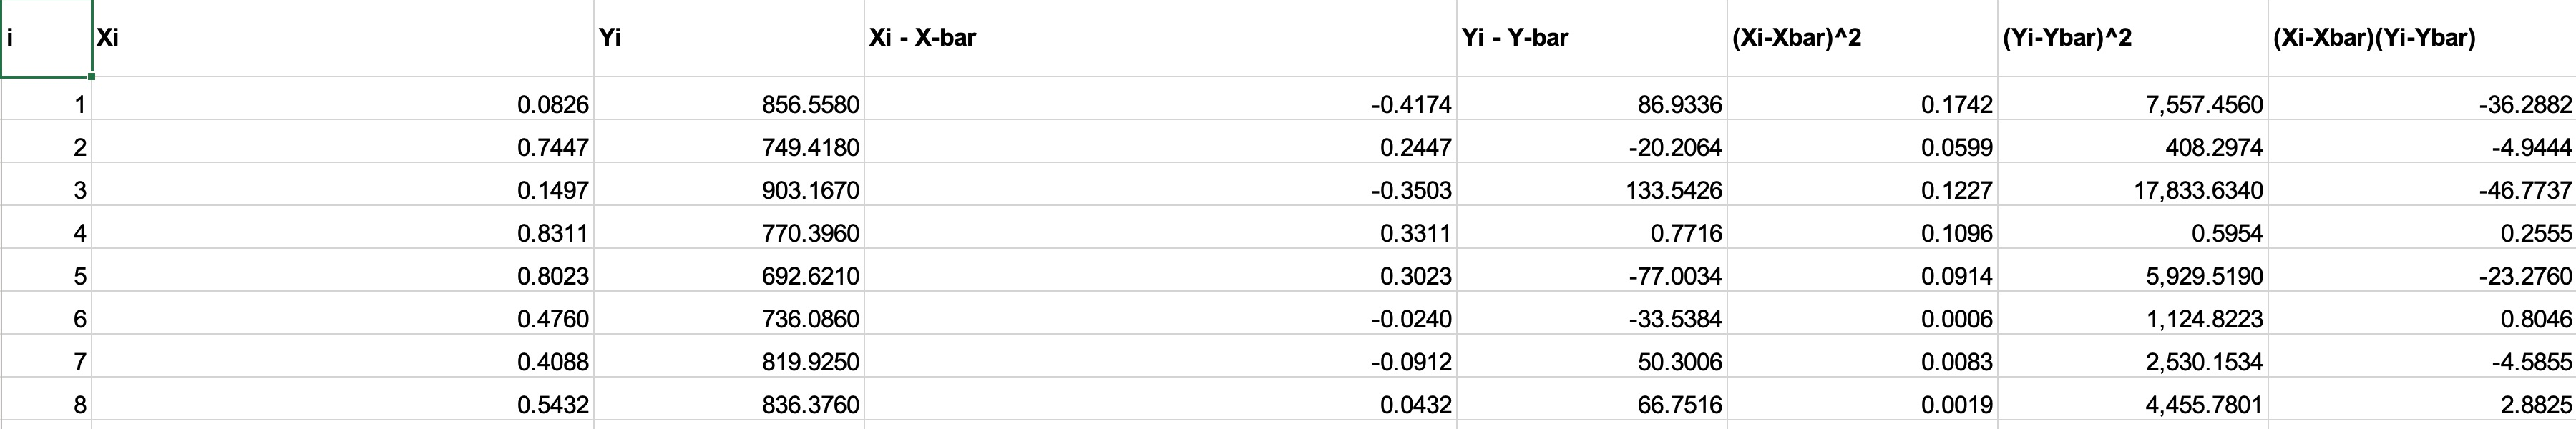
\includegraphics[width=\textwidth]{images/lecture4_excel_manual_deviations.png}
\begin{itemize}
\item Row 43: \texttt{D43=B43-\$C\$5} computes $X_1-\overline X$; \texttt{E43=C43-\$C\$6} computes $Y_1-\overline Y$.
\item Then square each deviation and multiply the two deviations: \texttt{F43=D43\^{}2}, \texttt{G43=E43\^{}2}, \texttt{H43=D43*E43}.
\item Copy down through row 142. The dollar signs keep the means fixed. Row 144 sums each column; both deviation sums are zero up to rounding.
\end{itemize}
\end{frame}

\begin{frame}{By Hand, Step 2: From Sums to the OLS Line}
\begin{center}
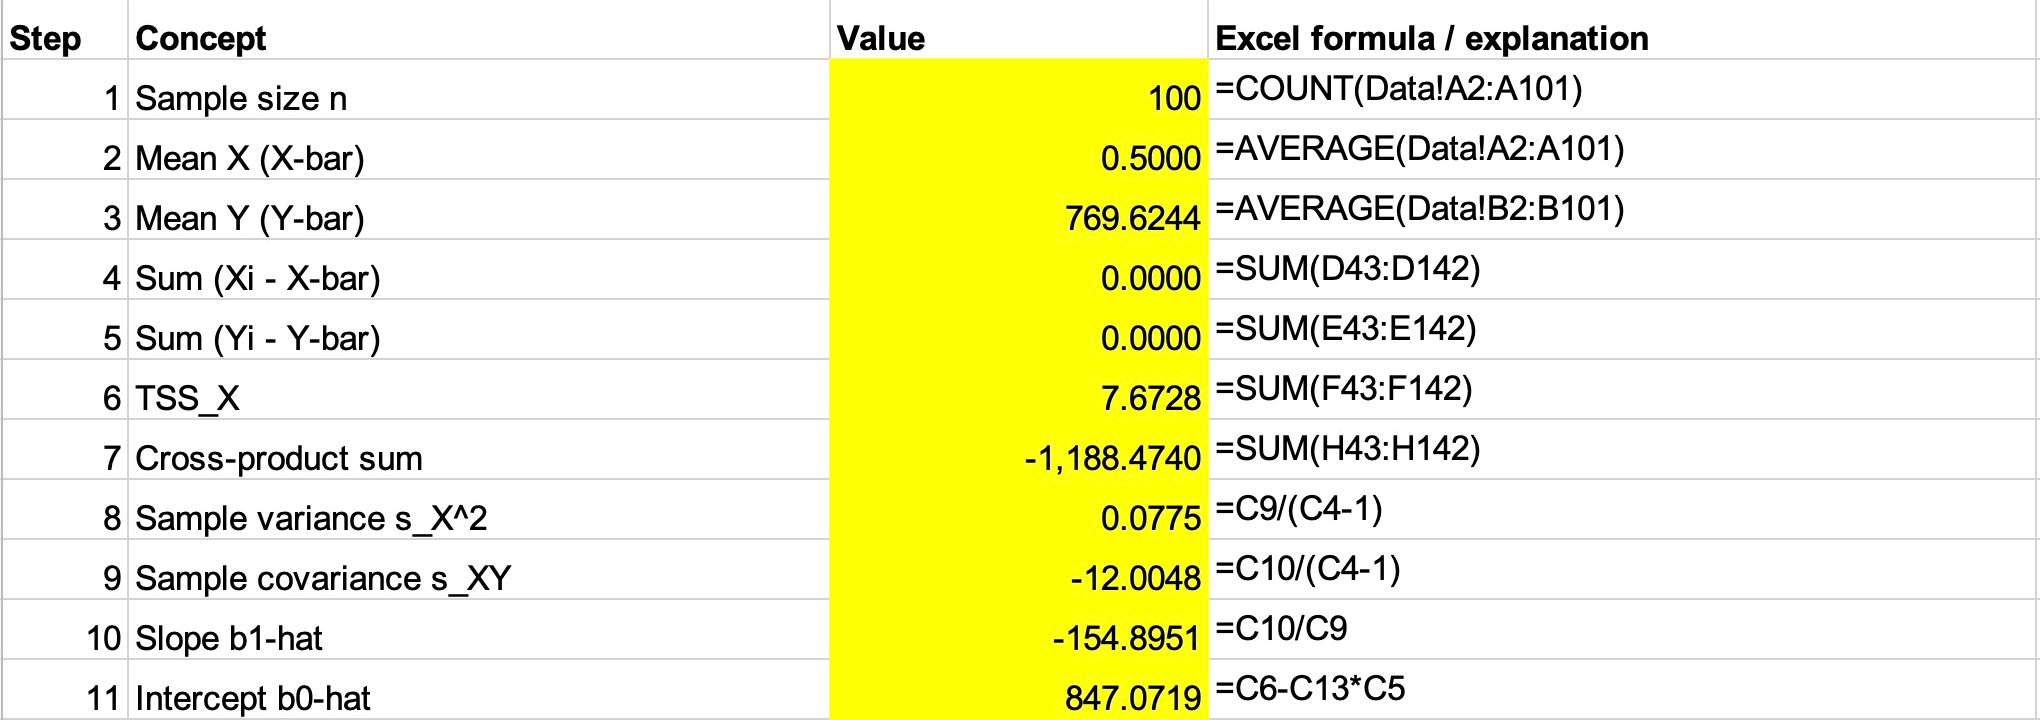
\includegraphics[width=.88\textwidth,height=2.7cm,keepaspectratio]{images/lecture4_excel_manual_means.png}
\end{center}
\small
Let $S_{XY}=\sum_i(X_i-\overline X)(Y_i-\overline Y)$ be the \textbf{cross-product sum}.
Then $s_{XY}=S_{XY}/(n-1)$ and $s_X^2=TSS_X/(n-1)$.
\begin{align*}
\widehat\beta_1&=\frac{S_{XY}}{TSS_X}=\frac{s_{XY}}{s_X^2}
=\frac{-1188.4740}{7.6728}=-154.8951,\\
\widehat\beta_0&=\overline Y-\widehat\beta_1\overline X
=769.6244-(-154.8951)(0.5000)=847.0719.
\end{align*}
Use \texttt{C13=C10/C9} and \texttt{C14=C6-C13*C5}. Keep full precision in the cells.
\end{frame}

\begin{frame}{By Hand, Step 3: Predictions, Fit, and Error Size}
\small
For the first observation (row 43), enter:
\begin{center}
\begin{tabular}{lll}
\toprule
Cell & Excel formula & Meaning\\
\midrule
I43 & \texttt{=\$C\$14+\$C\$13*B43} & $\widehat Y_i=\widehat\beta_0+\widehat\beta_1X_i$\\
J43 & \texttt{=C43-I43} & $\widehat u_i=Y_i-\widehat Y_i$\\
K43 & \texttt{=J43\^{}2} & $\widehat u_i^2$\\
L43 & \texttt{=(I43-\$C\$6)\^{}2} & $(\widehat Y_i-\overline Y)^2$\\
\bottomrule
\end{tabular}
\end{center}
Copy down through row 142. Sum column K for $SSR$, G for $TSS_Y$, and L for $ESS$.
\begin{center}
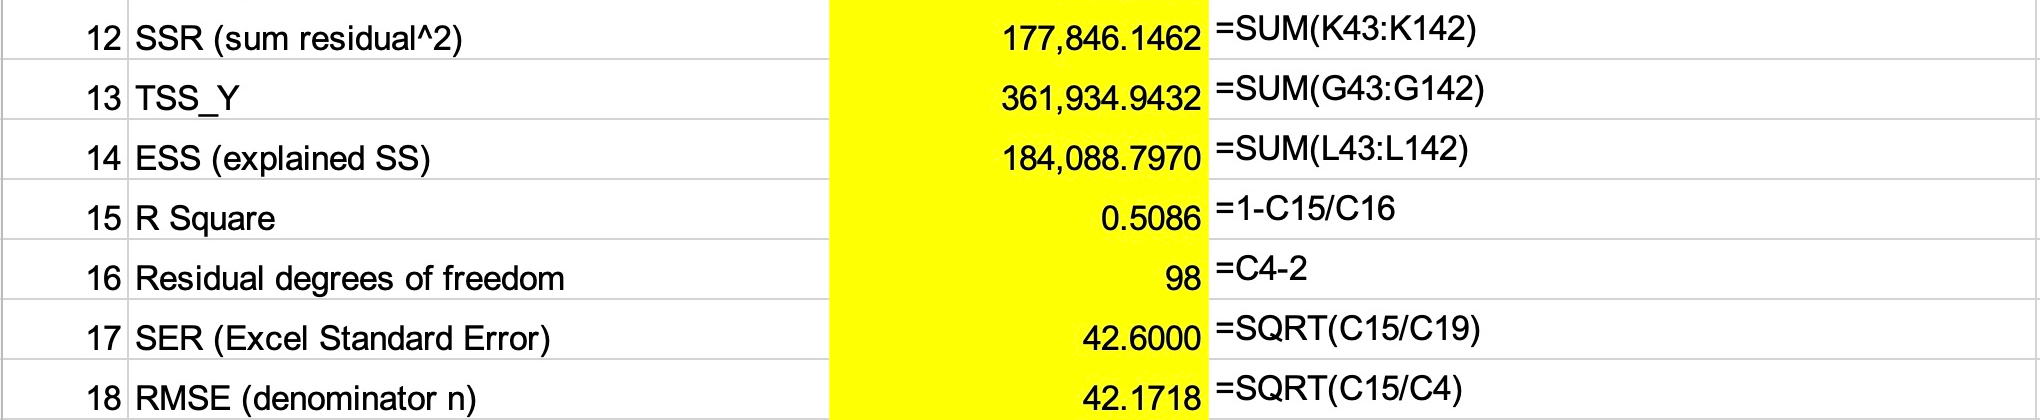
\includegraphics[width=.76\textwidth,height=2.6cm,keepaspectratio]{images/lecture4_excel_manual_fit.png}
\end{center}
Then calculate $R^2=1-SSR/TSS_Y$, $SER=\sqrt{SSR/98}$, and $RMSE=\sqrt{SSR/100}$.
\end{frame}

\begin{frame}{By Hand, Step 4: Standard Errors and $t$ Statistics}
\small
Under homoskedasticity, estimate the common error variance by $SER^2$:
\begin{align*}
SE(\widehat\beta_1)&=\frac{SER}{\sqrt{TSS_X}}
=\frac{42.6000}{\sqrt{7.6728}}=15.3792,\\
SE(\widehat\beta_0)&=SER\sqrt{\frac1n+\frac{\overline X^2}{TSS_X}}
=42.6000\sqrt{\frac1{100}+\frac{0.5000^2}{7.6728}}=8.7908.
\end{align*}
In \textbf{Paso\_a\_paso}, the formulas are:
\begin{itemize}
\item C22: \texttt{=C20/SQRT(C9)}; C23: \texttt{=C20*SQRT(1/C4+C5\^{}2/C9)}.
\item To test zero coefficients, divide each estimate by its own standard error:
\[
t_1=\frac{-154.8951}{15.3792}=-10.0717,\qquad
t_0=\frac{847.0719}{8.7908}=96.3594.
\]
\item C24: \texttt{=C13/C22}; C25: \texttt{=C14/C23}.
\end{itemize}
\end{frame}

\begin{frame}{By Hand, Step 5: $p$-Values and Confidence Intervals}
\small
A \textbf{$p$-value is a probability}: under $H_0$, how likely is a $t$ statistic at least this extreme in either direction?
\begin{center}
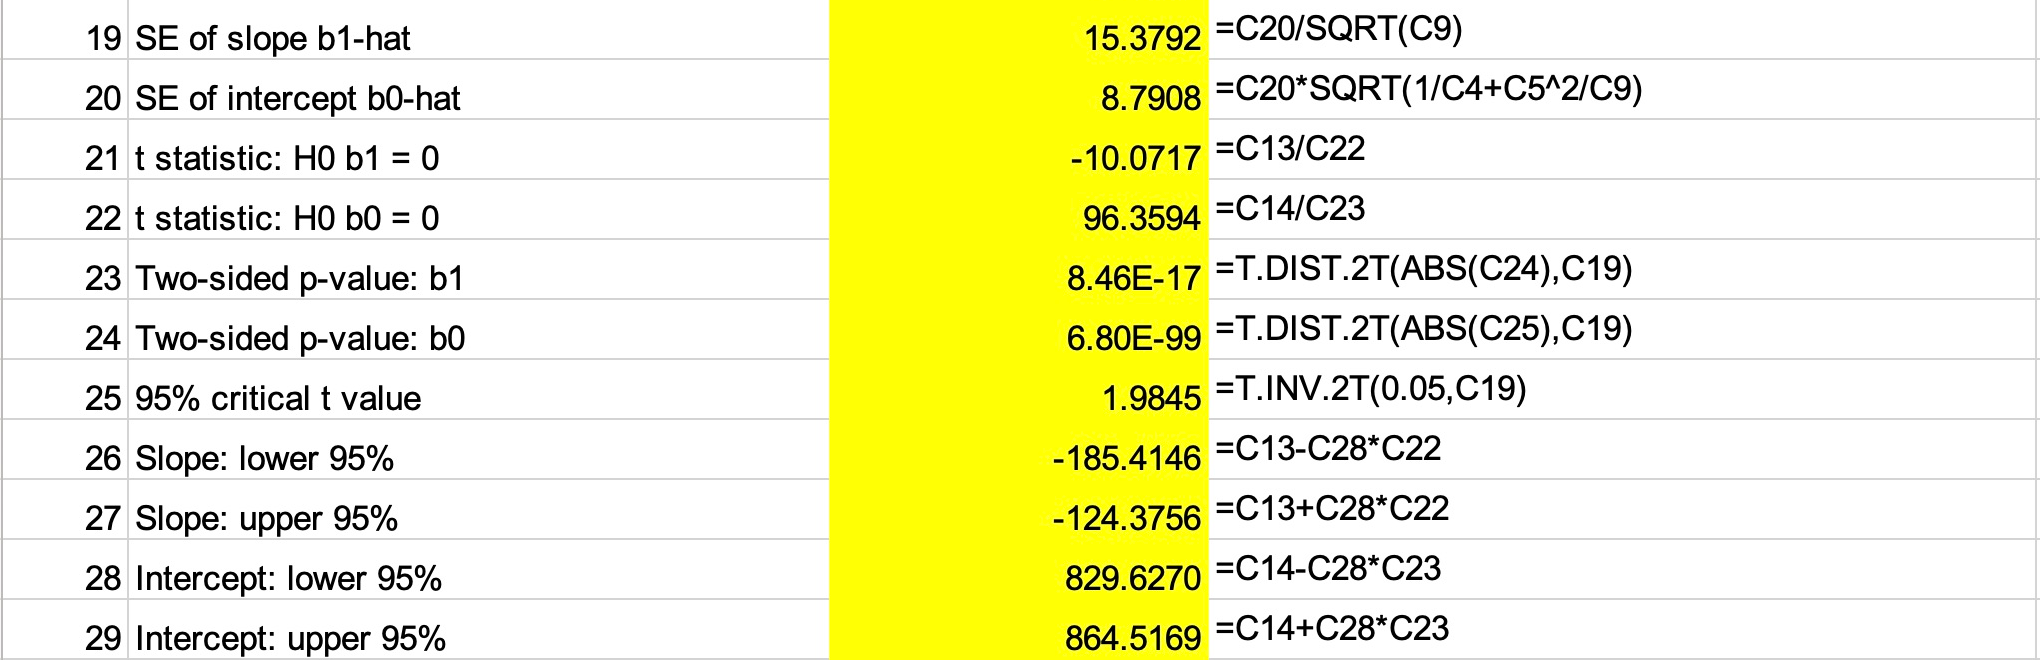
\includegraphics[width=.90\textwidth,height=2.6cm,keepaspectratio]{images/lecture4_excel_manual_inference.png}
\end{center}
\begin{columns}[T]
\begin{column}{.49\textwidth}
\textbf{Two-sided $p$-values ($df=98$)}
\begin{itemize}
\item Slope, C26:\\\texttt{=T.DIST.2T(ABS(C24),C19)}
\item Intercept, C27:\\\texttt{=T.DIST.2T(ABS(C25),C19)}
\end{itemize}
\end{column}
\begin{column}{.48\textwidth}
\textbf{95\% confidence intervals}
\begin{itemize}
\item Critical value, C28:\\\texttt{=T.INV.2T(0.05,C19)}
\item Use $\widehat\beta_j\pm\texttt{C28}\times SE(\widehat\beta_j)$.
\end{itemize}
\end{column}
\end{columns}
\medskip
{\footnotesize Yellow cells match ToolPak. Function names and separators may differ with Excel's language settings.}
\end{frame}


\begin{frame}
\frametitle{Homoskedasticity vs. Heteroskedasticity}

\begin{itemize}
    \item In regression analysis, we often make an important assumption about the variance of the error term, $u$, known as \textbf{homoskedasticity}.
    \item Homoskedasticity implies that the variance of the error term is constant for all observations.
    \item However, in most cases, this assumption may not hold, leading to \textbf{heteroskedasticity}, where the variance of $u$ varies across observations.
\end{itemize}
\begin{block}{Homoskedasticity vs. Heteroskedasticity}
For homoskedastic data, we assume:
\[
\text{var}(u_i \mid X) = \sigma^2 \quad \text{for all } i
\]

For heteroskedastic data, the variance of $u_i$ is not constant:
\[
\text{var}(u_i \mid X) = \sigma_i^2 \quad \text{for each } i
\]
\end{block}

\end{frame}


\begin{frame}{Graphical Illustration}
 \begin{columns}
\begin{column}{0.35\textwidth}
    \begin{itemize}
    \item Understanding \textbf{homoskedasticity} and heteroskedasticity is crucial in regression analysis.
    \item \textbf{Homoskedasticity} assumes constant error variance, while heteroskedasticity implies varying error variance.
    \item To account for heteroskedasticity, robust standard errors can be used to obtain valid inferences.
    \end{itemize}
\end{column}
\begin{column}{0.7\textwidth}
\begin{figure}
  \centering
         \vspace{-5mm}
        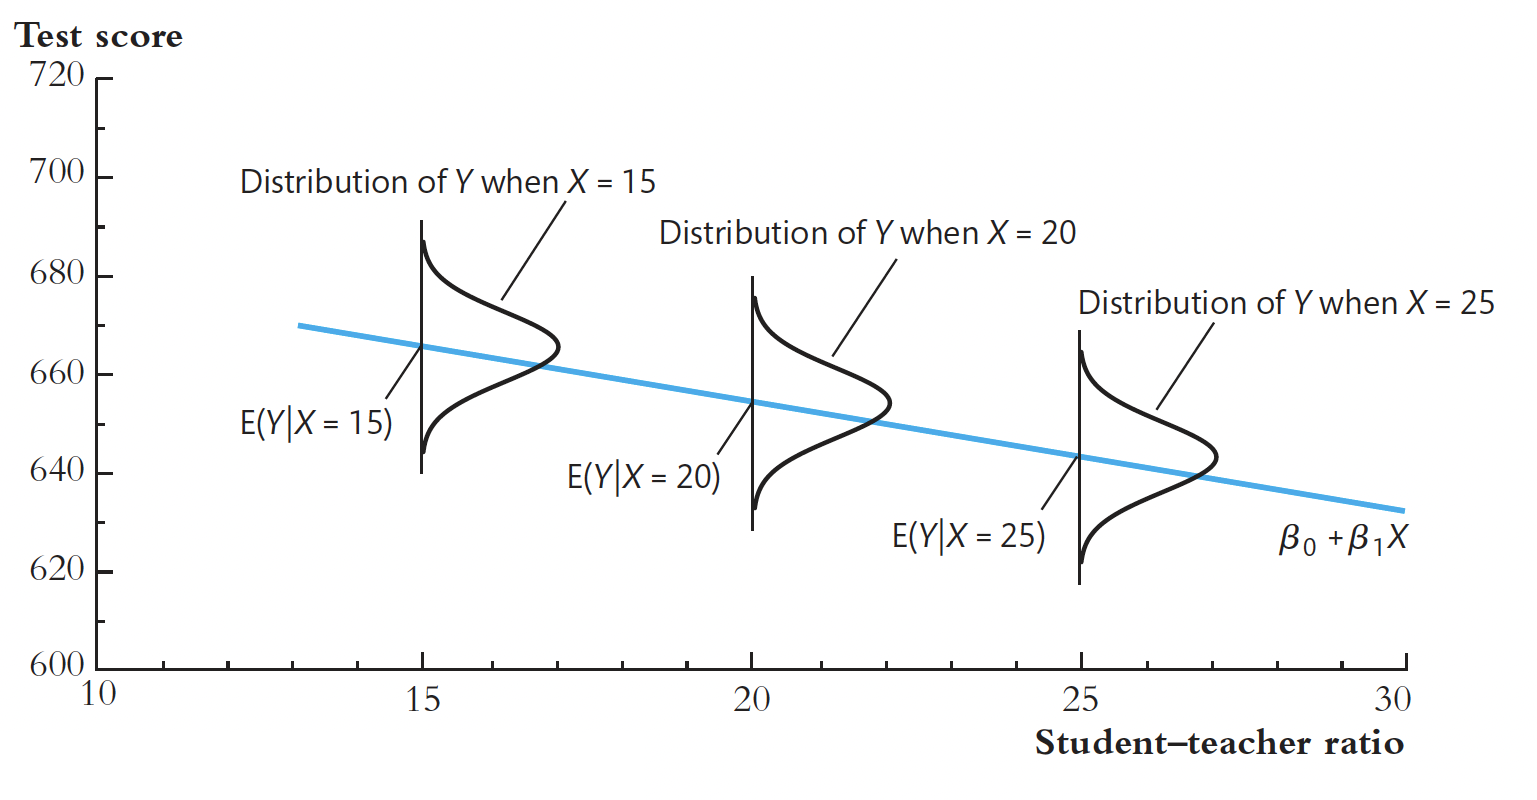
\includegraphics[scale=.35]{images/homoskedastic.png}
\end{figure}
\end{column}
\end{columns}
\end{frame}

\begin{frame}{Graphical Illustration}
 \begin{columns}
\begin{column}{0.35\textwidth}
    \begin{itemize}
    \item Understanding homoskedasticity and \textbf{heteroskedasticity} is crucial in regression analysis.
    \item Homoskedasticity assumes constant error variance, while \textbf{heteroskedasticity} implies varying error variance.
    \item To account for \textbf{heteroskedasticity}, robust standard errors can be used to obtain valid inferences.
    \end{itemize}
\end{column}
\begin{column}{0.7\textwidth}
\begin{figure}
  \centering
         \vspace{-5mm}
        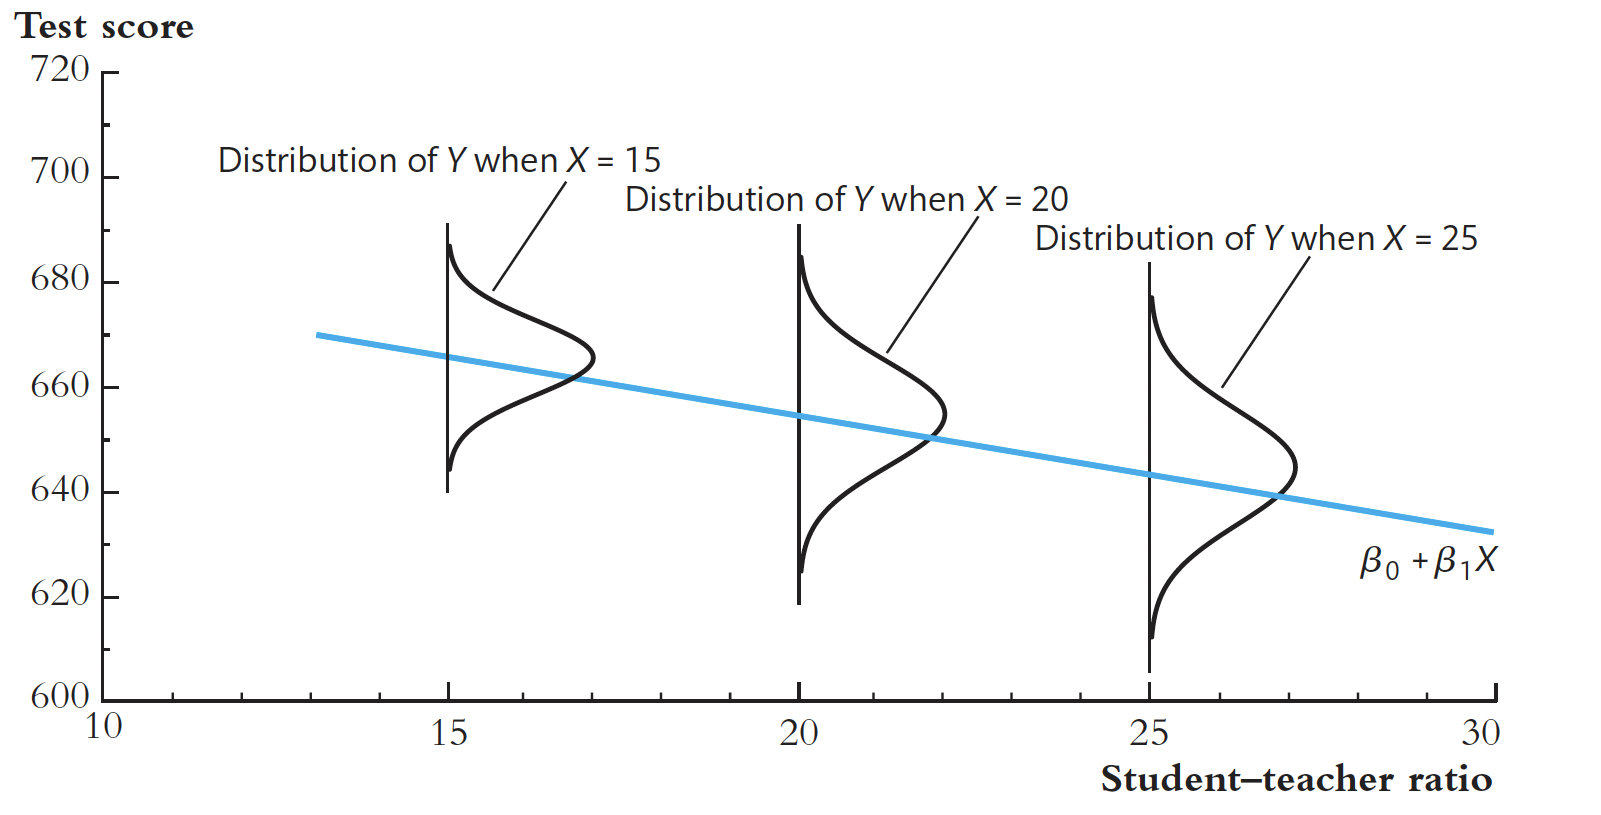
\includegraphics[scale=.35]{images/heteroskedastic.png}
\end{figure}
\end{column}
\end{columns}
\end{frame}

\begin{frame}{The Variance of the Slope with Heteroskedastic Errors}
\small
Write $TSS_X=\sum_i(X_i-\overline X)^2$. Conditional on all the regressors, the weights are fixed:
\[
\widehat\beta_1-\beta_1=\frac{\sum_i(X_i-\overline X)u_i}{TSS_X}.
\]
If errors are uncorrelated across observations conditional on $X$,
\begin{align*}
\operatorname{var}(\widehat\beta_1\mid X)
&=\frac{1}{TSS_X^2}\operatorname{var}\!\left(\sum_i(X_i-\overline X)u_i\mid X\right)\\
&=\frac{\sum_i(X_i-\overline X)^2\operatorname{var}(u_i\mid X)}{TSS_X^2}.
\end{align*}
Under homoskedasticity, $\operatorname{var}(u_i\mid X)=\sigma_u^2$, so this reduces to
$\sigma_u^2/TSS_X$. With heteroskedasticity, the observation-specific variances remain inside the sum.
\end{frame}

\begin{frame}{Estimate a Heteroskedasticity-Robust Standard Error}
\small
Use squared residuals to estimate each observation's contribution to the variance:
\[
\widehat{\operatorname{var}}_{\mathrm{HC1}}(\widehat\beta_1)
=\frac{n}{n-2}\,
\frac{\sum_i(X_i-\overline X)^2\widehat u_i^2}
     {\left[\sum_i(X_i-\overline X)^2\right]^2}.
\]
\begin{itemize}
\item The numerator allows the size of the error to vary with $X_i$.
\item The denominator is $TSS_X^2$: square the \emph{sum of squared deviations}.
\item $n/(n-2)$ is a degrees-of-freedom adjustment (HC1).
\item Take the square root to obtain the robust standard error. Robust inference is justified by large-sample results under the usual regularity conditions.
\end{itemize}
The OLS coefficient estimates do not change; their estimated uncertainty does.
\end{frame}

\begin{frame}{Excel in Practice: What the ToolPak Does Not Provide}
\begin{columns}[c]
\begin{column}{.49\textwidth}
\small
\begin{itemize}
\item The standard errors in our \textbf{Regression} sheet use the homoskedasticity formula.
\item The ToolPak Regression dialog has \textbf{no option for heteroskedasticity-robust standard errors}.
\item If error variance changes with $X$, use a separate robust calculation before interpreting $t$ tests and confidence intervals.
\end{itemize}
\end{column}
\begin{column}{.47\textwidth}
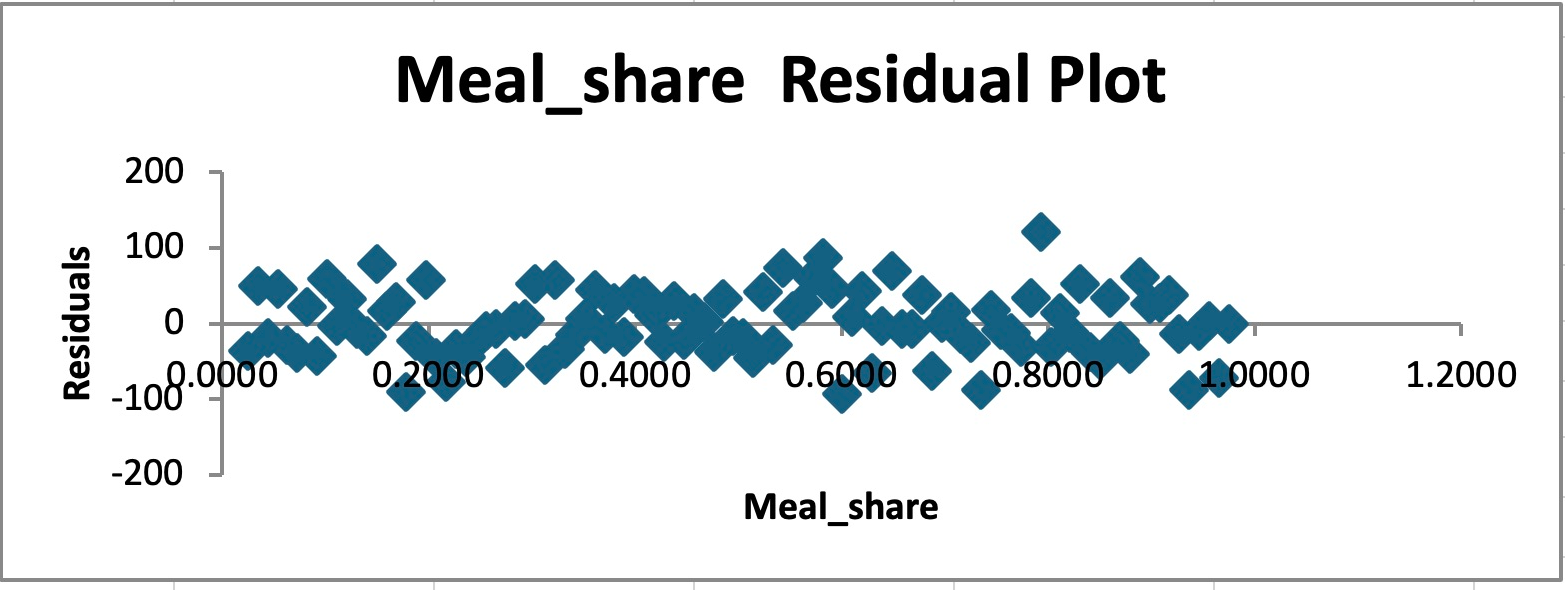
\includegraphics[width=\linewidth]{images/lecture4_excel_residual_plot.png}
\small
A residual plot helps diagnose changing spread. An absence of an obvious pattern does not establish constant variance.
\end{column}
\end{columns}
\end{frame}


\begin{frame}{The Theoretical Foundations of OLS}

Let us consider a linear regression model:

\[
Y_i = \beta_0 + \beta_1 X_{i}  + u_i
\]

Subject to the following assumptions:

\begin{enumerate}
    \item Zero Conditional Mean: The errors $u_i$ have a conditional mean of zero given the values of the independent variables, i.e., $\mathbb{E}(u_i|X_{i}) = 0$ for all $i$.

    \item Random Draws: observations $(Y_i;X_i)$ are randomly drawn from the same population distribution, i.e., they are i.i.d. for all $i$.
    
    \item Large outliers are rare: $\mathbb{E}(Y^4)<\infty$ and $\mathbb{E}(X^4)<\infty$
    
    \item Homoskedasticity: The errors have constant variance, i.e., $\text{Var}(u_i) = \sigma_u^2$ for all $i$.
    
    \item u is normally distributed: $u\sim\mathcal{N}(0;\sigma_u^2)$.
\end{enumerate}

\begin{exampleblock}{Gauss-Markov Theorem}
Under assumptions 1-4, the OLS estimators are Best Linear Unbiased Estimators (BLUE).
\end{exampleblock}
\end{frame}

\begin{frame}{The Gauss-Markov Theorem}
\begin{itemize}
    \item The OLS estimator $\hat{\beta}_1$ is a linear estimator, that is, it can be written as a linear function of $Y_1, ..., Y_n$:
    \begin{eqnarray*}
        &\hat{\beta}_1-\beta_1 = \frac{\sum_{i=1}^n (X_i - \overline{X})u_i}{\sum_{i=1}^n(X_i - \overline{X})^2}\equiv w^{OLS}_iu_i\\
        \text{where} &w^{OLS}_i=\frac{\sum_{i=1}^n (X_i - \overline{X})}{\sum_{i=1}^n(X_i - \overline{X})^2}
    \end{eqnarray*}
    \item The Gauss-Markov theorem states that among all possible choices of $\{w_i\}$ the OLS weights $w^{OLS}_i$ yield the smallest $var(\hat{\beta}_1)$.
    \item Under assumptions 1-5, the ordinary least squares (OLS) estimators $\hat{\beta}_0$ and $\hat{\beta}_1$  have the minimum variance among all (linear and non-linear) unbiased estimators
\end{itemize}
\end{frame}

\begin{frame}{The Gauss-Markov Theorem: Limits}
The Gauss-Markov Theorem is a crucial justification for using OLS in many regression analyses, but it is very restrictive and, therefore, has serious practical limitations.
\begin{itemize}
    \item The result is only for linear estimators –- only a small subset of estimators
    \item The condition of homoskedasticity often doesn’t hold (homoskedasticity is a special case)
    \item When estimating the population mean, if there are significant outliers, the median is preferred over the mean because it's less sensitive and has lower variance. Similarly, in regression, OLS estimators can also be sensitive to outliers. In such cases, other estimators like the Least Absolute Deviations (LAD) estimator may be more efficient:
    \begin{eqnarray*}
        \min_{\hat{\beta}_0;\hat{\beta}_1}\sum_{i=1}^n \mid Y_i - \beta_0 - \beta_1 X_i \mid 
    \end{eqnarray*}
\end{itemize}
\end{frame}


\begin{frame}{Back to the original question}
Suppose schools receive extra transfers from the central government so the share of subsidized school meals increases by 10\%-pt. What is the effect of this policy intervention (“treatment”) on test scores? 
\begin{itemize}
    \item This question requires an estimate of the causal effect on test scores of a change in the share of subsidized meals. Does our regression analysis using the California data set provide a compelling estimate of this causal effect?
    \item Not really – districts with a low share of subsidized meals tend to be ones with lots of other resources and higher income families, which provide kids with more learning opportunities outside school…this suggests that $corr(u_i; X_i)>0$ (that is, $\mathbb{E}(u_i\mid X_i)\neq 0$).
    \item It seems that we have omitted some factors, or variables, from our analysis, and this has biased our results…
\end{itemize}
\end{frame}


\begin{frame}[allowframebreaks]{Material}
\begin{itemize}
    \item[--] \textbf{Textbooks:}
    \begin{itemize}
        \item Introduction to Econometrics, 4th Edition, Global Edition, by Stock and Watson -- Chapter 5
    \end{itemize}
\end{itemize}
\end{frame}


\end{document}
